\chapter{Domain, Background and Problem Definition}
\label{chp:domain}

The problem of influence maximization starts with a set of nodes called \textit{seed}, this selection is either random, optimal, or based on certain heuristic \footnote{A problem solving method which may not provide optimal results, but are capable of producing close to the desired results.}. Each node in the seed is pre-activated, i.e. they are classified as nodes which have performed certain activity, or are already influenced by some phenomena. Then a process is simulated in which the seed nodes attempt to influence other nodes in their neighborhood to perform that same activity. This attempt is either successful or unsuccessful based on certain probability; if it turns out to be successful then the newly activated nodes also become active and repeat the same action of influencing their neighbors subsequently. Thus, a ripple effect is created which reaches and possibly influences all the nodes in a network. The main objective of influence maximization is to find out exactly which nodes are likely to maximize the spread, i.e. cause most nodes to become active.

	\section{Problem definition}
	\label{sec:domain-problem}
	In the introduction of chapter \ref{chp:intro} discusses the origin of the concept of influence with an example from social networks. In a social network, people are connected, which are described by the research community as "correlation". This correlation can be of three different types:
	
	\begin{itemize}
		\item Homophily: tendency of individuals to choose friends with similar characteristics \cite{mcpherson2001}.
		
		\item Confounding factors: external inspiration from the surrounding elements, or the environment.
		
		\item Influence: phenomenon that the action of individuals can induce their friends to act in similar way.
	\end{itemize}
	
	These correlations can be found by analyzing the structure of a network, as well as event logs of users, containing their \textit{actions}. An action is any activity performed by an individual, e.g. purchasing an item, sharing a link, tagging a photo, etc. Once an action is performed, the user performing it becomes \textit{active}. This means that if two users $u$ and $v$ are connected, then their property of being active is correlated with each other.
	
	Mathematically, if we have an undirected graph $G=(V,E)$ with nodes $V$ representing users and edges $E$ representing relation (optionally, their labels can refer to actions), then in a series of time stamps, each non-active node in $U={u_1,u_2,u_3\ldots}$ has a probability of being active, defined by probability function $p(x)\in [0,1]$. Here, $x$ is the number of active nodes in $V={v_1,v_2,v_3\ldots}$ with which the non-active node has an edge. Thus, the probability is dependent on active nodes in the connected neighbours.
	
	It is important to add that of the three stated sources of correlation, Influence is the only one which is not only correlation but causation \cite{mcpherson2001}. This has been proven by Anagnostopoulos et al. \cite{anagnostopoulos2008}. In their work, the authors did two experiments: \textit{Shuffle Test} and \textit{Edge Reversal Test}. In the first test, they proved a postulate that if the source of correlation is other than social influence, then shuffling of time steps does not affect user actions considerably. In their second test, they showed that since influence is unidirectional, then reverting the directions of edges will make significant change in propagation if the source of correlation is influence.
	
	The influence maximization (IM) problem is solved by the accurate selection of seed nodes, which are at the micro-level of a network. However it is imminent to know that a network can be studied on three scales and each scale is an important contributor when understanding a network. The next section describes these scales and comments on various properties, which are used in our experiments.
	
	
	\section{Macro-scale: structural properties of networks}
	\label{sec:domain-macro-scale}
	Structural properties are holistic level attributes of a network which explain the overall structure of a network. These properties help in classifying a network (e.g. scale-free, small-world, synchronized, etc.). Such properties have been extensively studied in past few decades and researchers have prescribed several ways to examine network structures, each method with its own significance:

	\begin{enumerate}
		%TODO: Find a book on graph theory and cite it whenver a new term is introduced in the document.
		
		\item Format: defines whether a network is directed or undirected. A directed network assumes that edges are unidirectional vectors between nodes. A directed edge from node $u$ to $v$ strictly means that $u$ is connected to $v$, it does not say $v$ is also connected to $u$. In case of undirected networks, edges are bidirectional. In our experiments, all graphs are of undirected format.		
		
		\item Weight: in a weighted network, each edge carries certain numeric value describing the significance of that particular edge. Weight can be certain probability, frequency, or other measure. If all edges have uniform weight in a network, it is considered as unweighted.
		
		\item Size (nodes): the number of total nodes in the network. The size of the network is primary metric which defines the scale.
		
		\item Edges: the number of links between nodes in the network. The greater number of edges make a graph dense and provides more channels for information to flow from one node to another.
		
		\item Average Degree: arithmetic mean of the number of edges per node in a network. Higher average degree indicates one of two things, i.e. either a big proportion of nodes are densely connected, or there exist some outlier hub nodes which are highly connected. A network with low Average Degree is not necessarily weak.
		
		\item Highest Degree: the maximum number of edges a particular node has in the network. It's sometimes denoted with $\Delta(G)$. Naturally lowest degree is denoted with $\delta(G)$\footnote{In this document, $\delta$ is not used to represent lowest degree, instead it represents \textit{gain} as discussed in \ref{chp:proof}}. However, lowest degree is majorly ignored as in almost every complex network, $\delta(G)=1$.
				
		\item Assortativity: Pearson correlation coefficient of nodes at any side of an edge. Ranging between -1 and 1, negative value means that the high degree nodes tend to connect with low degree nodes, positive value means that the nodes connect with respect to degree similarity.
		
		\item Triad Count: number of 3 interconnected nodes. Also referred as Triangles, this structural property is quite significant in complex networks because it directly impacts the strength of a network. The higher the triad count, the stronger (resilient) a network is.
		
		\item Power-law exponent ($\alpha$): in a scale free network, power-law coefficient describes how \textit{skewed} the curve in the degree-distribution plot is. Generally, this value varies between 2-3 for majority of social networks.
		
		\item Average Path Length (APL): the average minumum number of edges between shortest paths among nodes, given as $l\dfrac{1}{n(n-1)}\sum_{i,j}d_{i,j}$ where $i,j$ is any pair of nodes, $l$ is the number of nodes in the path between $i$ and $j$ and $n$ is total number of nodes in the network. Real complex networks have low APL. For example in small-world networks, nodes are connected with every other nodes through an APL of 6 or less. %TODO: add reference to 6-degree of separation
		
		\item Clustering Coefficient (CC): ratio of number of Triads connected to a node to possible number of Triads\cite{watts1998}.
		
		\item Transitivity (Global CC): Cliqueness of a network given as $C_{global}=\dfrac{3\times |triads|}{|possible_triads|}$.
		
		%\item Wedge Count: this property was introduced much later in the field \cite{seshadhri2013}. Wedge count is the number of paths with 2 edges. In larger networks, this is useful in counting the number of triads. However, its significance in broader applications is debatable.
		
		%\item Square Count: analogous to Triad count, it is the number of 4 interconnected nodes. Its use is very limited because of high cost to compute this number on larger networks, and also because Triad count already fulfills the same need which Square count proposes.
			
		\item Diameter (longest Geodesic): number of edges in longest path that exists from two most distinct nodes. Lower value of diameter suggests that the network is in form of a large cluster. Larger values indicate sparse graph.
		
		\item Density: the ratio between existing network edges and all possible edges among nodes.
		
		\item Community: a strongly connected induced sub-graph within a network. Communities are identified using a variety of methods. Not all scale-free networks have community structure, but almost all social networks have it. Presence of community plays significant role when dealing with heterogeneous networks as well as application of divide and conquer techniques on a large scale network.
		
	\end{enumerate}
	
	In experiments presented in this document, the scope was restricted to only the most widely used attributes, which include: Size, Edges, Average Degree, APL, Diameter, Transitivity, Assortativity and $\alpha$. However, wherever necessary, other properties are also indicated to support discussions and interpretations of the experimental results.
	

	\section{Micro-scale: Node properties and seed selection methods}
	\label{sec:domain-micro-scale}
	This is the granular level of a network, where properties of individual nodes are discussed. Since in a complex network, each node has its own significance and changing a few handpicked nodes can greatly impact the whole network, therefore there are many metrics available to analyze a node significance.
	
	In the influence mining process, the target is to choose a seed set and researchers have proposed various methods to select these seed nodes, and these methods can be broadly categorized into five groups:	
	
	\begin{enumerate}
		\item Topological methods: choose the seed nodes based on the structure of a network. Some nodes are very well connected in the network whereas others are loosely connected with other nodes. This associates an inherent importance to nodes due to their own connectivity as well as the connectivity of their direct neighbors.  %a  regions of a network, while some lie in the outskirts; a few nodes occur frequently during interactions between other nodes, while there will be some which are distinct.
		
		\item Simulation based methods: perform Monte Carlo simulations \footnote{A process which is repeated many times with a random selection of data. After numerous repetitions, the scenarios which happen more frequently are obtained.} to discover influential nodes in iterative manner. They provide guarantees of effectiveness within certain approximation of the best possible solution, but often fail to scale on large data sets due to the time and space complexity.
		
		\item Sampling methods: focus on identifying seed nodes via some statistical sampling method, either in single pass or in an iterative manner. The difference is that in the single pass methods, the sample of seed nodes is drawn at once, while in the iterative method, a single node or a small set of nodes is removed and the process repeats on remaining connected network.
			
		\item Community focused methods: use a divide and conquer technique. These methods first divide the network into clusters or communities using various methods, then choose seed nodes from within these communities. This way, the seed selection process can be scaled to larger networks.

		\item Scoring methods: assign a score to each node via some scoring method and select the subset of nodes with higher scores as seed. Such methods are quite effective when used on particularly friendly types of networks which are tailor made for a specific use case. %For example, famous Pagerank algorithm \cite{pagerank1999} was designed to rank web pages.
		
	\end{enumerate}

	
	\section{Information diffusion}
	\label{sec:domain-diffusion-models}
	The idea of diffusion is rooted in Epidemics. There are people infected by a certain virus or bacteria, and people who are susceptible to being infected. Some of the infected people are recovered or cured. The first and basic model of diffusion is called SI (Susceptible-Infected) model proposed by Pastorsatorras \cite{pastor2001}. The process of influence spread is actually a diffusion of information process based on SI-model, i.e. when an event is triggered on seed nodes, how is the information about that event spread to the remaining of network. There are two foundational models to observe the information diffusion process (\cite{domingos2001,richardson2002,goldenberg2001}) which are discussed below:
	
		\subsection{Linear threshold model (LT)}
		In this model, the information flow is observed from the perspective of the recipient node, i.e. the node which is inactive and will be influenced by its neighbours. The target node will have a certain threshold. If the influence of the active neighbours exceeds the threshold, then this node will also be triggered.

		\subsection{Independent cascade model (IC)}
		In this model, the flow of information is observed from the perspective of active nodes which will influence other nodes. Each active node spreads the information to its neighbourhood independently, i.e. without considering what other active nodes are doing, or what happened in the previous iterations.
		
		\subsection{Other models}
		On the basis of the foundation models, some other variants have also caught attention in literature. A few examples are enlisted in the following:
		
		\begin{enumerate}
			\item Weighted cascade model (WC): an extension to IC model with an added feature that the probability of a seed node to make its neighbouring nodes respond to the event information. This probability is calculated using the in-degree of potential nodes \cite{kempe2003}.
			
			\item Trivalency model: chooses a uniform probability between 0.1, 0.01, 0.001; this is the probability with which an individual seed node spreads the event information to its neighbour nodes \cite{chen2010}.
			
			\item Unanimous Threshold Model: this extends the LT model and adds a very strict idea that each node is highly resistant to influence and thus its activation threshold is equal to its total degree \cite{chen2009b}.
		\end{enumerate}


	\section{Diffusion process convergence}
	\label{sec:domain-convergence}
	Convergence defines when the diffusion process stops. There is only one method to halt the diffusion process, i.e. when the seed set is identified. For example, in a network of 100 nodes if the budget $k=5$ then five node are selected as seed set through some heuristic and the diffusion process is simulated on this seed set. When the propagation stops or covers entire network, then the process is said to have converged and the total number of influenced nodes is obtained as influence quantity. This parameter is provided as input to influence process and cannot be changed once set, except as a special case of Online influence maximization \cite{lei2015}, which is because in the online process, all nodes in the network are not visited at once but rather some nodes are attempted to be influenced, and based on their feedback the next set of nodes is chosen for activation.
	

	\section{Generalized view}
	\label{sec:domain-generalized-view}
	There are various components to the influence mining problem, some of which have been discussed and more will be covered later in the discussion. While the influence mining problem is subjective and depends highly on the area of application, there are three core features which are necessary to encompass this idea as a generalized model:
	
	\begin{enumerate}
		\item Seed selection: the process of identifying a set of influential nodes $S$ using an algorithm $M$.
		
		\item Diffusion or spread: the estimated number of inactive nodes, which were influenced by the seed set after completion of simulation process; note that there can be a single trial as well as several trials in a simulation. This is denoted by $\sigma(S)$.
		
		\item Convergence: external deciding factor which quantifies the information diffusion or influence, and halts the process. Typically, when all nodes in the seed nodes stop spreading the influence further, the influence process is said to be converged with an output parameter $\sigma$, which is the measure of influence spread.
	\end{enumerate}


	\section{Synthetic networks. Why are they used?}
	\label{sec:domain-synthetic-nets}
	The field of Influence Maximization uses real-world networks for real-world applications unsurprisingly. Therefore the basic optics suggests to use real networks for influence maximization experiments. However, it is not always plausible to collect, synthesize and use real networks due to many reasons.
	
	For example, famous Social networking website, Facebook was reported to have 2.6 billion monthly active users in first quarter of 2020 \cite{nasdaq2020}, i.e. the network size is 2.6 billion nodes. A network this large is impossible to process in realistic time even on the most powerful data centers. Even if attempted, the time it will take to execute even the fastest influence maximization method available will be so much that the original network would have been altered in the midst.
	
	Size is not the only factor, take DBLP \footnote{Digital Bibliography \& Library Project is a German website hosting a database of over 4.8 million research articles.} as an example. The co-authorship network extracted by this database contains disconnected components, which require pre-processing in order to apply influence maximization.
	
	Third reason is uniqueness of each network. Even in social media, Facebook's network is quite different than the famous microblogging website, Twitter, as shown by Hashmi et al. \cite{hashmi2012} that not all social networks are structurally equal.
	
	To address such complications, the researchers make use of \textit{Synthetic networks}. Synthetic networks are not collected or extracted from real-world data. They are generated by providing certain algorithms with tuneable parameters. For example, random network (see \ref{chp:intro}) based on Erdös–Rényi model \cite{erdos1960} inputs two parameters: $n$ as the size of the network to generate and $p$ as the probability of edge formation between nodes. Similarly, Barabási-Albert model adds preferential attachment \footnote{Phenomenon that the nodes tend to connect with other nodes with a preference, i.e. high-degree nodes tend to form new edges with other high-degree nodes.} parameter to grow the network in discrete time steps \cite{barabasi1999}.
	
	These synthetic networks are used for multiple reasons:
	
	\begin{enumerate}
		\item Test and evaluate new network analysis methods without real-world bias.
		
		\item As default data set to compare with the graphs extracted from real-world data.  		
		\item Identify the class of a real network by matching the statistics with existing synthetic networks with known characteristics. For example if a synthetic network is drawn using Watts model \cite{watts1998}, then a real-world network which has similar clustering coefficient and short APL will indicate that the two networks are comparable.
		
		\item Construct an ideal scenario in which the network is in clean, pre-processed form. For example, if some desired experiment is meant to be run on a complete network with community structure, then a synthetic network generator can provide such data.
		
		\item In some cases, the real network data is not available, for example due to privacy concerns. Synthetic networks work as substitute in such cases.
	\end{enumerate}

Throughout this thesis, we have used both real world networks as well as synthetic networks, as and when needed during experiments.
	

	\section{Network dismantling and resilience}
	\label{sec:domain-resilience}
	The term Resilience in network sciences is understood as tendency of a network to remain intact, such that it stays functional even if some nodes are removed. The higher the resilience, the more difficult it is to dismantle the network through random and targeted attacks\footnote{A targeted attack is when one or more nodes pre-selected by the attacker are attacked in a network in order to maximize the damage.}. This term is also synonymous in computer networks, where fault tolerance is a critical subject. Sterbenz et. al. \cite{sterbenz2011} define resilience as "the ability of the network to provide desired service even when challenged by attacks, large-scale disasters, and other failures". The subject has been extensively studied in computer networks, especially in the context of Internet security but has recently caught attention in diverse applications, including mobile networks, social networks, transport networks, and more. 
	
	The problem of network dismantling coexists -- and sometimes confused -- with decycling problem. The objective is to identify and remove the nodes such that the graph becomes acyclic, thus a node is connected with other nodes in exactly one path. The resultant graph after network decycling has $n-1$ edges, and if any edge is removed then the graph breaks into two sub-graphs. Similarly, introducing a new edge between existing nodes make the graph cyclic. The matter under discussion is strictly about network dismantling, and decycling is only used as a technique to dismantle the network such as in \cite{braunstein2016}. The relation between network dismantling and resilient node identification is the constraint $k$; the objective is to find a set of $k$ most resilient nodes which, when removed, dismantle the largest component of target network to the maximum extent possible. Meaning that if there are 100 nodes in a graph and $k=5$ nodes are to be removed, then the network dismantling problem is identifying the best set of five nodes such that if they are removed, the maximum number of edges are removed.
	
	Although there seems to be a clear segregation in past literature between resilience and influence studies, we found that both are interestingly interlinked, as discussed in chapter \ref{chp:inf-framework} in detail. \\


	\section{Influence process illustration}
	A typical influence process can be seen in figure \ref{fig:influence-process} in which a network is passed as input and based on certain iterative or non-iterative algorithm a set of seed nodes is selected. These seed nodes are then tested via inflence test or resilience test and finally the influence of the seed set is returend. Additionally, a simulation is presented in discrete steps in figure \ref{fig:ic-simulation} which tells how the diffusion process takes place in Independent cascade model as an example.
	% Source diagram here: https://drive.google.com/file/d/1AMVqRqj-GDfIZuTEUTv5SPkjt5gtoe_g/view?usp=sharing
	\begin{figure}[H]
		\centering
		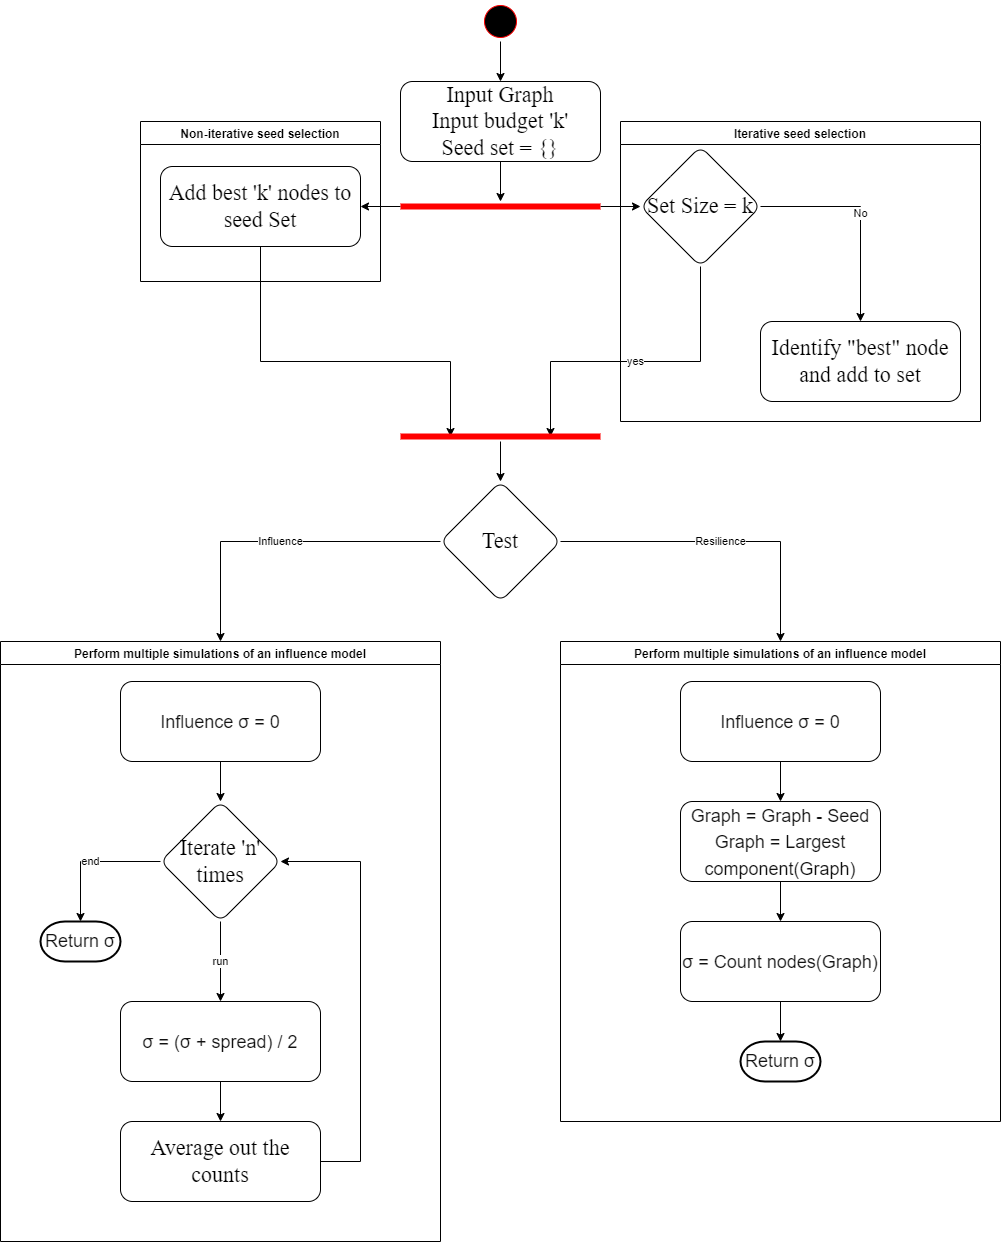
\includegraphics[width=0.7\textwidth]{influence-process}
		\caption[Influence process flow diagram]{Illustration of influence process. The function inputs a network and returns the influence measure $\sigma$ of seed nodes selected in the process.}
		\label{fig:influence-process}
	\end{figure}
	
	% Source diagram here: https://drive.google.com/file/d/1AMVqRqj-GDfIZuTEUTv5SPkjt5gtoe_g/view?usp=sharing
	\begin{figure}[H]
		\centering
		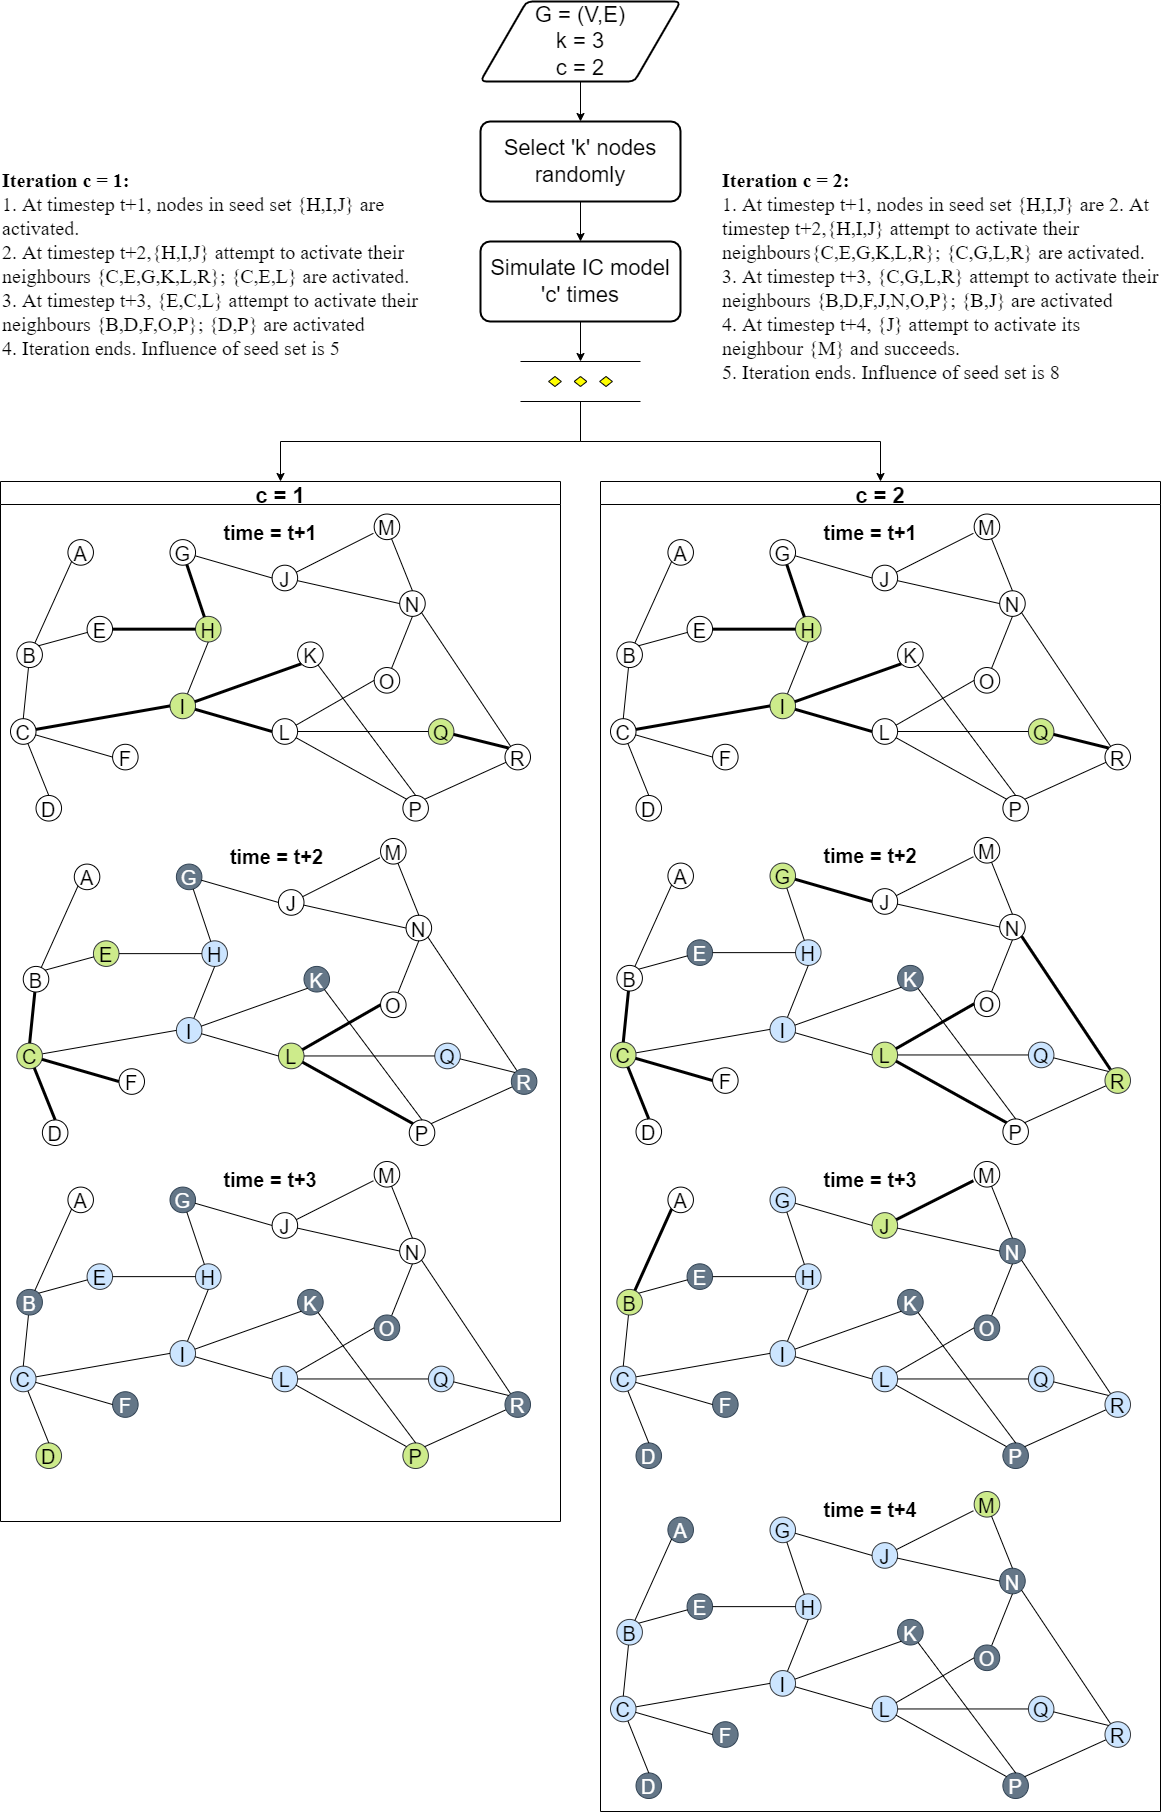
\includegraphics[width=1.0\textwidth]{ic-simulation}
		\caption[Information diffusion simulation under IC model]{An example explaining how diffusion process takes place in IC model in a graph. The two simulations shown are averaged out to give the average influence spread $\sigma$.}
		\label{fig:ic-simulation}
	\end{figure}


	\section{Summary}
	Influence maximization under any of the commonly used diffusion models is NP-hard for approximate value of spread, as given in Chapter \ref{chp:proof}; thus, these cannot be used ingenuously with real networks, because the computation time they take is too high due to the size of the network and its tendency to change dynamics rapidly, such as formation of community structure, or shortening the paths between distinct nodes, etc. Therefore, the aim should be to look for data mining approaches (such as clustering for community detection, or classification to classify nodes) for computation of influence of nodes in a complex network, so that the most influential ones can be spotted. The data mining techniques are likely to perform well because such algorithms can learn from existing state of data and adapt. For example, a straightforward approach to detect communities can be to construct fixed groups of nodes of fixed size with dense links. A data mining algorithm on the other hand will not only identify flexible sized networks, but also find hierarchies, i.e. communities within a large community. Thus this document terms the phenomenon of mining the influential nodes from a network as \textit{Influence Mining}, over the more commonly used term of Influence Maximization \cite{vahidipour1920}. \\
	
This chapter presented the fundamental concepts required to comprehend the problem of influence mining. The next chapter further capitalizes these concepts and covers the necessary details and related work in various areas.
